\documentclass{xmu-beamer}
% \xmubeamerdebuglayouttrue % 调试用
% Presentation metadata.
\title[Short Title]{Main Title of Your Presentation}
\subtitle{Subtitle}
\author{Philoso}
\institute[人工智能系·信息学院·厦门大学]{人工智能系, \newline 信息学院, \newline 厦门大学.}
\date{\today}

\addbibresource{reference.bib}
\usepackage{listings}
\lstset{
    basicstyle=\ttfamily\footnotesize,
    keywordstyle=\color{PrussianBlue},
    commentstyle=\color{gray},
    stringstyle=\color{NeonCarrot},
    numbers=left,
    numberstyle=\tiny\color{gray},
    frame=single,
    rulecolor=\color{LightGrayishBlue},
    backgroundcolor=\color{Solitude},
    showstringspaces=false,
    breaklines=true,
    tabsize=4
}

\begin{document}

\maketitlepage

\begin{frame}[t]{Overview}
    \tableofcontents
\end{frame}

% Basic content examples.
\makesection{Basic blocks}

\begin{frame}{中文测试}
    \textrm{这是中文}

    \textsf{这是中文}

    \texttt{这是中文}

    \textrm{This is English text.}

    \textsf{This is English sans-serif text.}

    \texttt{This is English monospaced text.}
\end{frame}

\begin{frame}[fragile]{Code Listing}
    \begin{lstlisting}[language=Python]
def normalize_scores(scores):
    """Scale a list of scores to the range [0, 1]."""
    # 中文注释
    lo = min(scores)
    hi = max(scores)
    if hi == lo:
        return [0.0 for _ in scores]

    return [(score - lo) / (hi - lo) for score in scores]

values = [72, 88, 91, 67]
print(normalize_scores(values))
    \end{lstlisting}
\end{frame}

\begin{frame}{Bullet Points}
    \begin{itemize}
        \item Lorem ipsum dolor sit amet, consectetur adipiscing elit
        \item Aliquam blandit faucibus nisi, sit amet dapibus enim tempus eu
        \item Nulla commodo, erat quis gravida posuere pellentesque
        \item Vestibulum faucibus velit a augue condimentum quis convallis nulla gravida
    \end{itemize}
\end{frame}

\begin{frame}{Numbered List}
    \begin{enumerate}
        \item Lorem ipsum dolor sit amet, consectetur adipiscing elit
        \item Aliquam blandit faucibus nisi, sit amet dapibus enim tempus eu
        \item Nulla commodo, erat quis gravida posuere pellentesque
        \item Vestibulum faucibus velit a augue condimentum quis convallis nulla gravida
    \end{enumerate}
\end{frame}

\begin{frame}{Blocks of Highlighted Text}
    Important text can be marked with \alert{alert color}.

    \begin{block}{Block}
        Sample text.
    \end{block}

    \begin{alertblock}{Alert Block}
        Sample text in an alert block.
    \end{alertblock}

    \begin{exampleblock}{Example Block}
        Sample text in an example block.
    \end{exampleblock}
\end{frame}

\begin{frame}{Multiple Columns}
    \begin{columns}
        \begin{column}{0.45\textwidth}
            \colheader{Heading}
            \begin{enumerate}
                \item Statement
                \item Explanation
                \item Example
            \end{enumerate}
        \end{column}
        \begin{column}{0.45\textwidth}
            \colheader{Heading}
            Lorem ipsum dolor sit amet, consectetur adipiscing elit. Integer lectus nisl, ultricies in feugiat rutrum, porttitor sit amet augue.
        \end{column}
    \end{columns}
\end{frame}

\begin{frame}{Table}
    \begin{table}
        \begin{tabular}{l l l}
            \toprule
            \textbf{Treatments} & \textbf{Response 1} & \textbf{Response 2} \\
            \midrule
            Treatment 1         & 0.0003262           & 0.562               \\
            Treatment 2         & 0.0015681           & 0.910               \\
            Treatment 3         & 0.0009271           & 0.296               \\
            \bottomrule
        \end{tabular}
        \caption{Table caption}
    \end{table}
\end{frame}

% Mathematical statements and graphics.
\makesection{Theorems and Figures}

\begin{frame}{Theorem}
    \begin{theorem}[Mass--energy equivalence]
        $E = mc^2$
    \end{theorem}
    Equation in text:
    \begin{equation}
        c^{2} = a^{2} + b^{2}
    \end{equation}
\end{frame}

\begin{frame}{Figure}
    \begin{figure}
        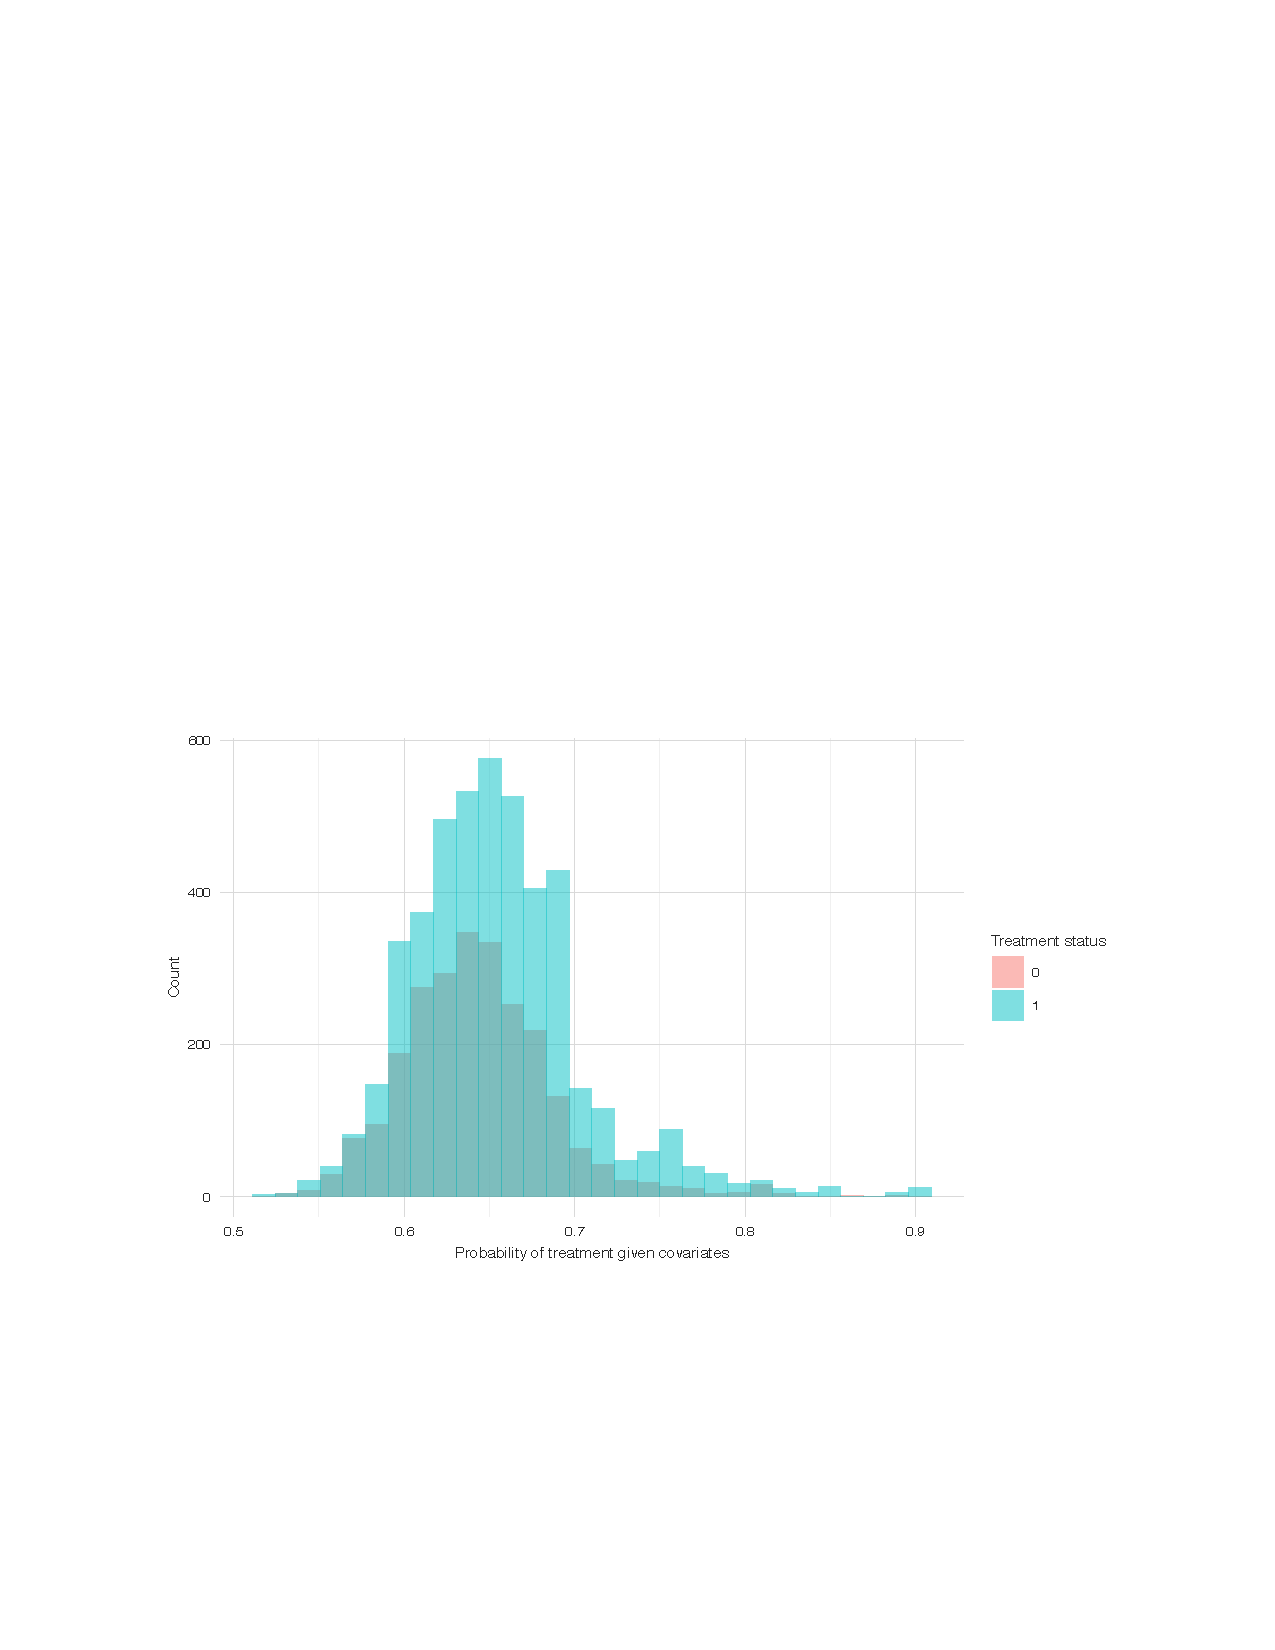
\includegraphics[height=0.5\paperheight]{figures/results_fig.pdf}
        \caption{Figure caption}
    \end{figure}
\end{frame}

\begin{frame}{Wrapped Figure}
    \begin{wrapfigure}{r}{0.4\textwidth}
        \centering
        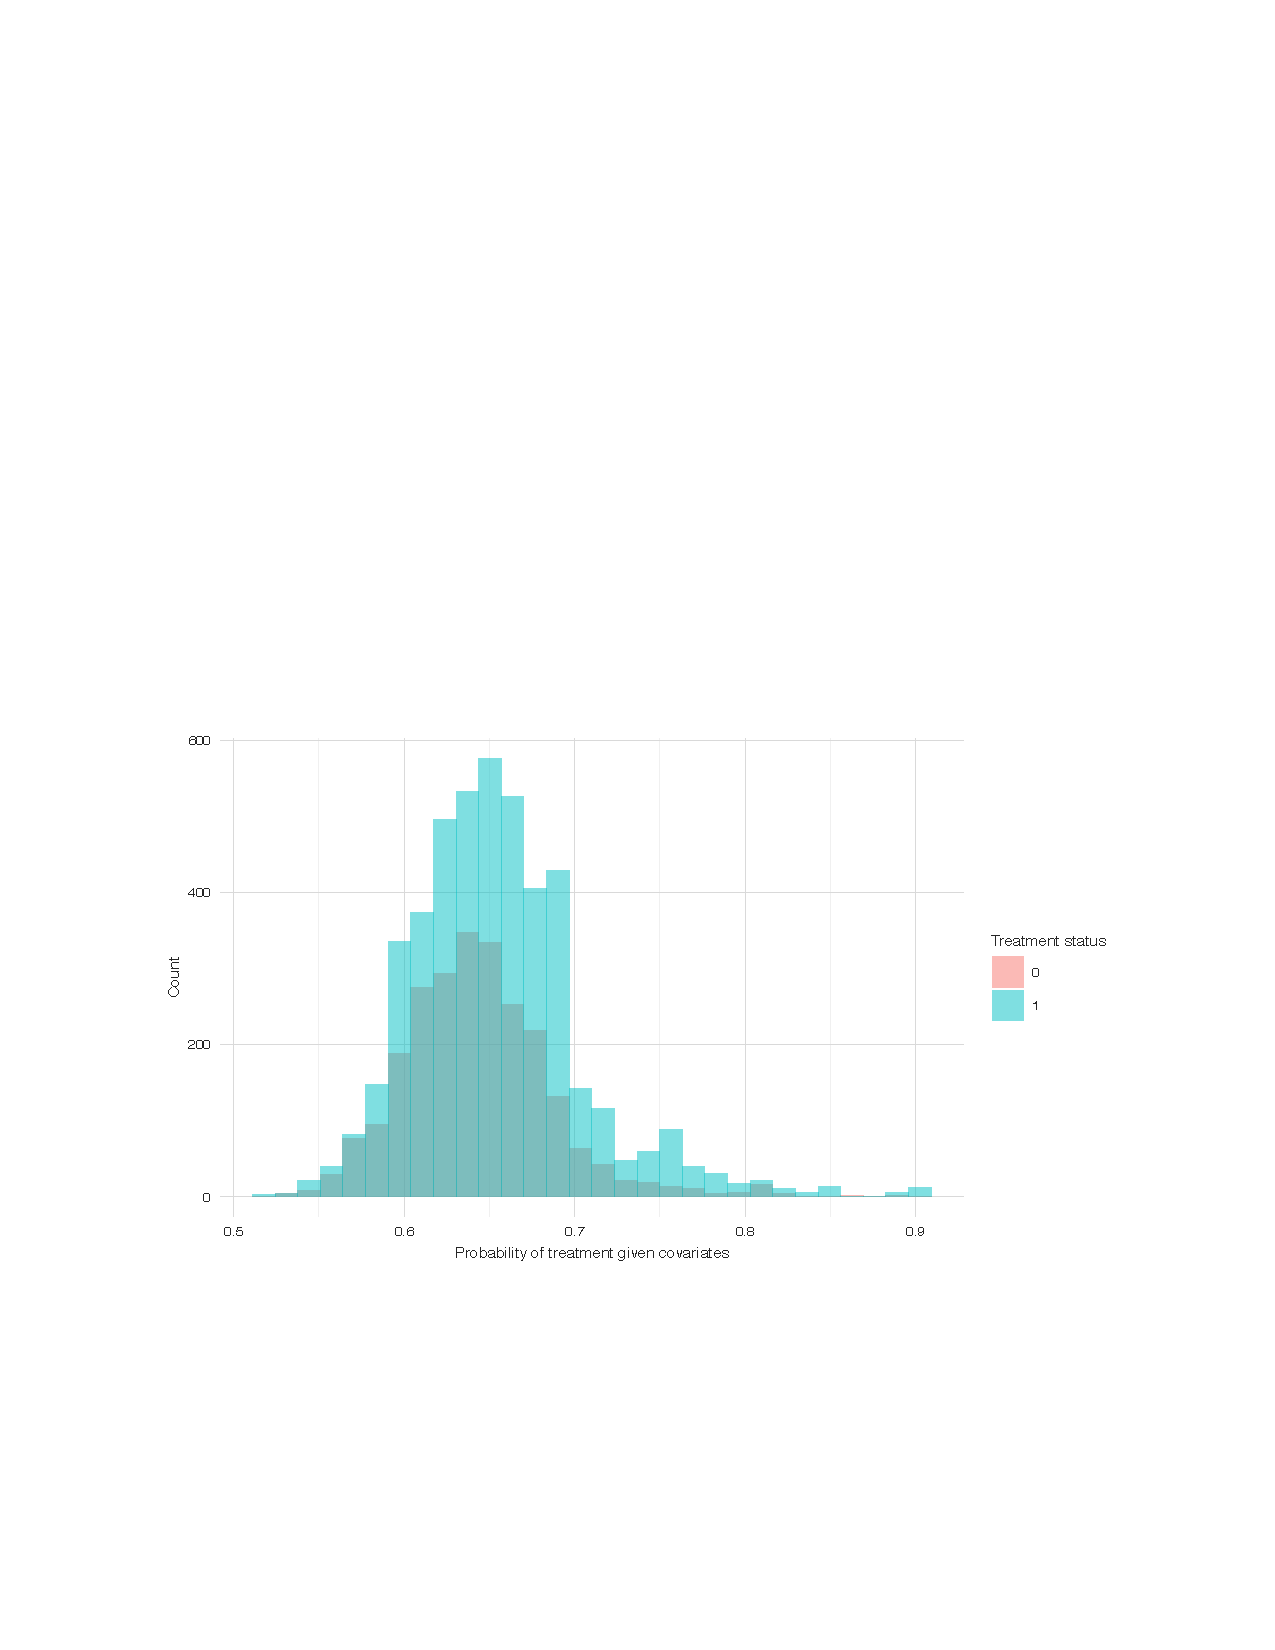
\includegraphics[width=0.4\textwidth]{figures/results_fig.pdf}
        \caption{Figure caption}
    \end{wrapfigure}
    Lorem ipsum dolor sit amet, consectetur adipiscing elit, sed do eiusmod tempor incididunt ut labore et dolore magna aliqua. Duis aute irure dolor in reprehenderit in voluptate velit esse cillum dolore eu fugiat nulla pariatur.
\end{frame}

% Citations and bibliography.
\makesection{Citations and References}

\begin{frame}[fragile]{Citation}
    An example of the \verb|\cite| command to cite within the presentation:\\~

    This statement requires citation\cite{Radford2021clip}.
\end{frame}

\begin{frame}[allowframebreaks]{References}
    \footnotesize
    \printbibliography
\end{frame}

\finalpagetext{Thank you for your attention}
\makefinalpage

\end{document}
